\chapter{Ranking and Recommendation} 
\label{cha:AHP}
In this chapter we propose a technique that aids in network QoS-aware selection of cloud services for provisioning mobile (or device with internet access but limited processing capability and storage), real-time and interactive applications.
We build upon our previous work in Chapter \ref{cha:cocoon}, where we have developed an automated approach, along with a unified domain model capable of fully describing infrastructure services in Cloud computing. 
This approach will take into account real-time, variable network QoS constraints.
It not only allows users to compare and select a cloud service based on a single criterion (e.g. total cost, max size limit for storage, memory size for compute instance), but also supports 
a utility function that combines multiple selection criteria pertaining to storage, compute, and network services.

\section{The Problem of Selecting Optimal Service Configuration}
\label{sec:TheProblemOfSelectingOptimalServiceConfiguration}
While the elastic nature of cloud services makes it suitable for provisioning all kinds of applications, the heterogeneity of cloud service configurations and their distributed nature raises some serious technical challenges. 
The cloud computing landscape is evolving with multiple and diverse options for compute (also known as virtual machines) and storage services. Hence, application owners are facing a daunting task when trying to select cloud services that can meet their constraints. According to Burstorm \cite{Burstorm} there are over 426 of various compute and storage service providers with deployments in over 11,072 locations. Even within a particular provider there are different variations of the services. For example, Amazon Web Service (AWS) has 674 different offerings differentiated by price, QoS features and location. Add to this every quarter they add about 4 new services, change business models (price and terms) and sometimes even add new locations. To be able to select the best mix of service offering from an abundance of possibilities, application owners must simultaneously consider and optimize complex dependencies and heterogeneous sets of criteria (price, features, location, QoS etc.). For instance, it's not enough to just select optimal cloud storage service, corresponding computing capabilities are essential to guarantee that one is able to process the data as fast as possible while minimizing the cost.

\subsection{Ambiguous Terminologies}
Ambiguous terminologies are often used to describe similar configurations,
for instance different units of measurements are used for similar metrics.
We performed unit conversions during instantiation of
concepts to simplify the discovery process.

For example, an Amazon EC2 Micro Instance has 613 MB
of memory which is converted to approximately 0.599 GB. Another example is the
CPU clock speed. Amazon refers to it as “ECUs”\cite{AmazonEC2}:
“\textit{One EC2 Compute Unit provides the equivalent COMPUTE capacity of a 1.0-1.2 GHz 2007 Opteron or 2007 Xeon processor. This is also the equivalent to an early-2006 1.7 GHz Xeon processor referenced in our original documentation}”.
In 2007, AMD and Intel released both dual-core and quad-core models of the Opteron and Xeon chips, respectively. So it is obviously not clear what an Amazon EC2 Compute Unit compares to. To eliminate this ambiguity, we obtained the compute service clock speed by trying out the actual instance under Linux OS and run \texttt{more /proc/cpuinfo} on it.

\subsection{Varied Price Model}
Another example of disparity between different Cloud providers is the price model of “on Demand instances”. GoGrid’s plan, although having a similar concept to Amazon’s On Demand and Reserved Instance, gives very little importance to what type or how many of compute services a user is deploying. GoGrid charges users based on what they
call RAM hours – 1 GB RAM compute service deployed for 1 hour consumes 1 RAM Hour. A 2 GB RAM compute service deployed for 1 hour consumes 2 RAM Hour.
It is worthwhile mentioning that only Azure clearly states that one month is considered to have 31 days. This is important as the key advantage of the fine grained pay-as-you-go price model which, for example, should charge a user the same when they use 2GB for
half a month or 1 GB for a whole month. 
Other vendors merely give a GB-month price
without clarifying how short term usage is handled. It is neither reflected in their usage
calculator. We chose 31 days as default value in calculation.

Regarding storage services, providers charge for every operation that an application
program or user undertakes. These operations are effected on storage services via
RESTful APIs or Simple Object Access Protocol (SOAP) API. Cloud providers refer to
the same set of operations with different names, for example Azure refers to storage
service operations as transactions. Nevertheless, the operations are categorized into
upload and download categories as shown in Table \ref{table:request_types_across_storage_services}.
Red means an access fee is charged;
green means the service is free; and yellow means access fees are not specified,
and can usually be treated as green/free of charge. To facilitate our calculation of similar
and equivalent requests across multiple providers, we analyzed and pre-processed the
price data, recorded it in our domain model and used a homogenized value in the CloudRecommender. For example, Windows Azure Storage
charges a flat price per transaction. It is considered as transaction whenever there is a
“touch” operation, i.e. Create, Read, Update, Delete (CRUD) operation over the RESTful
service interface, on any component (Blobs, Tables or Queues) of Windows Azure Storage.

\begin{table}[htbp]
\resizebox{\textwidth}{!}{
\setlength{\arrayrulewidth}{1.5pt}
\begin{tabular}{|l|l|l|l|l|}
\hline
                                    &                                    & \multicolumn{3}{l|}{\textbf{Requests}}                                                                                                       \\ \cline{3-5} 
\multirow{-2}{*}{\textbf{Provider}} & \multirow{-2}{*}{\textbf{Storage}} & \textbf{Upload}                                        & \textbf{Download}                                  & \textbf{Other}                 \\ \hline
\textbf{Windows Azure}              & Azure Storage                      & \cellcolor[HTML]{FD6864}storage transactions           & \cellcolor[HTML]{FD6864}storage transactions       & \cellcolor[HTML]{FFFC9E}       \\ \hline
\textbf{Amazon}                     & S3                                 & \cellcolor[HTML]{FD6864}PUT, COPY, POST, or LIST Reque & \cellcolor[HTML]{FD6864}GET and all other Requests & \cellcolor[HTML]{9AFF99}Delete \\ \hline
\textbf{GoGrid}                     & Cloud Storage                      & \multicolumn{3}{l|}{\cellcolor[HTML]{9AFF99}Transfer protocols such as SCP, SAMBA/CIFS, and RSYNC}                                           \\ \hline
\textbf{RackSpace}                  & Cloud Files                        & \cellcolor[HTML]{9AFF99}PUT, POST, LIST Requests       & \multicolumn{2}{l|}{\cellcolor[HTML]{9AFF99}HEAD, GET, DELETE Requests}             \\ \hline
\textbf{Nirvanix}                   & CSN                                & \cellcolor[HTML]{FFFC9E}                               & \cellcolor[HTML]{FD6864}Search                     & \cellcolor[HTML]{FFFC9E}       \\ \hline
\textbf{Ninefold}                   & Cloud Storage                      & \multicolumn{2}{l|}{\cellcolor[HTML]{FD6864}GET, PUT, POST, COPY, LIST and all other transactions}          & \cellcolor[HTML]{FFFC9E}       \\ \hline
\textbf{SoftLayer}                  & Object Storage                     & \multicolumn{3}{l|}{\cellcolor[HTML]{9AFF99}Not Specified/Unknow}                                                                            \\ \hline
\textbf{AT and T Synaptic}          & Storage as a Service               & \multicolumn{3}{l|}{\cellcolor[HTML]{9AFF99}Not Specified/Unknow}                                                                            \\ \hline
\end{tabular}
}
\caption{
    Depiction of configuration heterogeneities in request types across storage services.
    \colorbox{red}{Red} means an access fee is charged;
    \colorbox{green}{green} means the service is free;
    and \colorbox{yellow}{yellow} means access fees are not specified,
    and can usually be treated as free of charge.
}
\label{table:request_types_across_storage_services}
\end{table}

We collected service configuration information from a number of public Cloud providers (e.g., Windows Azure, Amazon, GoGrid, RackSpace, Nirvanix, Ninefold, SoftLayer, AT and T Synaptic, Cloud Central, etc.) to demonstrate the generic nature of the domain model with respect to capturing heterogeneous configuration (see Table \ref{table:configuration_heterogeneities}) information of infrastructure services. 

\begin{table}[htbp]\scriptsize\centering
\setlength{\arrayrulewidth}{1.5pt}
\begin{tabular}{llllllll}
\hline
& Compute & \makecell[l]{Pay As\\ You Go} & & Storage & \makecell[l]{Pay As\\ You Go} &  & Trail \\ 
\cline{2-3} \cline{5-6} \cline{8-8} 
\multirow{-2}{*}{Provider} & Terminology & Unit & \multirow{-2}{*}{\makecell[l]{Other\\ Plans*}} & Terminology & Unit  & \multirow{-2}{*}{\makecell[l]{Other\\ Plans*}} & \makecell[l]{Period\\ or Value} \\ 
\hline
\makecell[l]{Windows\\ Azure} & \cellcolor[HTML]{9AFF99}{\renewcommand{\arraystretch}{1}\begin{tabular}{@{}l@{}}Virtual\\ Server\end{tabular}} & \cellcolor[HTML]{9AFF99}/hr & \cellcolor[HTML]{9AFF99}1 & \cellcolor[HTML]{9AFF99}{\renewcommand{\arraystretch}{1}\begin{tabular}{@{}l@{}}Azure\\Storage\end{tabular}}  & \cellcolor[HTML]{9AFF99}{\renewcommand{\arraystretch}{1}\begin{tabular}{@{}l@{}}/GB\\month\end{tabular}} & \cellcolor[HTML]{9AFF99}1 & \cellcolor[HTML]{9AFF99}90 day \\
\hline
\makecell[l]{Amazon} & \cellcolor[HTML]{9AFF99}{\renewcommand{\arraystretch}{1}\begin{tabular}{@{}l@{}}EC2\\Instance\end{tabular}} & \cellcolor[HTML]{9AFF99}/hr & \cellcolor[HTML]{9AFF99}2 & \cellcolor[HTML]{9AFF99}{\renewcommand{\arraystretch}{1}\begin{tabular}{@{}l@{}}S3\end{tabular}}  & \cellcolor[HTML]{9AFF99}{\renewcommand{\arraystretch}{1}\begin{tabular}{@{}l@{}}/GB\\month\end{tabular}} & \cellcolor[HTML]{9AFF99}2& \cellcolor[HTML]{9AFF99}1 year \\
\hline
\makecell[l]{GoGrid} & \cellcolor[HTML]{9AFF99}{\renewcommand{\arraystretch}{1}\begin{tabular}{@{}l@{}}Cloud\\Servers\end{tabular}} & \cellcolor[HTML]{9AFF99}/RAM hr& \cellcolor[HTML]{9AFF99}1 & \cellcolor[HTML]{9AFF99}{\renewcommand{\arraystretch}{1}\begin{tabular}{@{}l@{}}Cloud\\Storage\end{tabular}}  & \cellcolor[HTML]{9AFF99}{\renewcommand{\arraystretch}{1}\begin{tabular}{@{}l@{}}/GB\\month\end{tabular}} & \cellcolor[HTML]{FD6864}& \cellcolor[HTML]{FD6864} \\
\hline
\makecell[l]{RackSpace} & \cellcolor[HTML]{9AFF99}{\renewcommand{\arraystretch}{1}\begin{tabular}{@{}l@{}}Cloud\\Servers\end{tabular}} & \cellcolor[HTML]{9AFF99}/RAM hr& \cellcolor[HTML]{9AFF99}\cellcolor[HTML]{FD6864} & \cellcolor[HTML]{9AFF99}{\renewcommand{\arraystretch}{1}\begin{tabular}{@{}l@{}}Cloud\\Files\end{tabular}}  & \cellcolor[HTML]{9AFF99}{\renewcommand{\arraystretch}{1}\begin{tabular}{@{}l@{}}/GB\\month\end{tabular}} & \cellcolor[HTML]{FD6864}& \cellcolor[HTML]{FD6864} \\
\hline
\makecell[l]{Nirvanix} & \cellcolor[HTML]{FD6864} & \cellcolor[HTML]{FD6864}& \cellcolor[HTML]{FD6864} & \cellcolor[HTML]{9AFF99}{\renewcommand{\arraystretch}{1}\begin{tabular}{@{}l@{}}CSN\end{tabular}}  & \cellcolor[HTML]{9AFF99}{\renewcommand{\arraystretch}{1}\begin{tabular}{@{}l@{}}/GB\\month\end{tabular}} & \cellcolor[HTML]{FD6864}& \cellcolor[HTML]{FD6864} \\
\hline
\makecell[l]{Ninefold} & \cellcolor[HTML]{9AFF99}{\renewcommand{\arraystretch}{1}\begin{tabular}{@{}l@{}}Virtual\\Server\end{tabular}} & \cellcolor[HTML]{9AFF99}/hr& \cellcolor[HTML]{FD6864} & \cellcolor[HTML]{9AFF99}{\renewcommand{\arraystretch}{1}\begin{tabular}{@{}l@{}}Cloud\\Storage\end{tabular}}  & \cellcolor[HTML]{9AFF99}{\renewcommand{\arraystretch}{1}\begin{tabular}{@{}l@{}}/GB\\month\end{tabular}} & \cellcolor[HTML]{9AFF99}1 & \cellcolor[HTML]{9AFF99}50 AUD\\
\hline
\makecell[l]{SoftLayer} & \cellcolor[HTML]{9AFF99}{\renewcommand{\arraystretch}{1}\begin{tabular}{@{}l@{}}Cloud\\Servers\end{tabular}} & \cellcolor[HTML]{9AFF99}/hr& \cellcolor[HTML]{9AFF99}1 & \cellcolor[HTML]{9AFF99}{\renewcommand{\arraystretch}{1}\begin{tabular}{@{}l@{}}Object\\Storage\end{tabular}}  & \cellcolor[HTML]{9AFF99}{\renewcommand{\arraystretch}{1}\begin{tabular}{@{}l@{}}/GB\end{tabular}} & \cellcolor[HTML]{FD6864} & \cellcolor[HTML]{FD6864}\\
\hline
\makecell[l]{AT and T\\Synaptic} & \cellcolor[HTML]{9AFF99}{\renewcommand{\arraystretch}{1}\begin{tabular}{@{}l@{}}Compute\\as a\\Service\end{tabular}} & \cellcolor[HTML]{9AFF99}{\renewcommand{\arraystretch}{1}\begin{tabular}{@{}l@{}}vCPU per hour\\+/RAM hr\end{tabular}}& \cellcolor[HTML]{FD6864} & \cellcolor[HTML]{9AFF99}{\renewcommand{\arraystretch}{1}\begin{tabular}{@{}l@{}}Storage\\as a\\Service\end{tabular}}  & \cellcolor[HTML]{9AFF99}{\renewcommand{\arraystretch}{1}\begin{tabular}{@{}l@{}}/GB\\month\end{tabular}} & \cellcolor[HTML]{FD6864} & \cellcolor[HTML]{FD6864}\\
\hline
\makecell[l]{Cloudcentral} & \cellcolor[HTML]{9AFF99}{\renewcommand{\arraystretch}{1}\begin{tabular}{@{}l@{}}Cloud\\Servers\end{tabular}} & \cellcolor[HTML]{9AFF99}/hr& \cellcolor[HTML]{FD6864} & \cellcolor[HTML]{FD6864} & \cellcolor[HTML]{FD6864} & \cellcolor[HTML]{FD6864} & \cellcolor[HTML]{FD6864}\\
\hline
\multicolumn{8}{l}{* Other Plans includes Monthly/Quarterly/Yearly Plan, Reserve and Bidding Price Option}
\end{tabular}
\caption{Depiction of configuration heterogeneities in compute and storage services
across providers. \magenta{Red blank cells} in the table mean that a configuration parameter is
\magenta{not supported}.
Some providers offer their services under a different pricing scheme than pay-as-
you-go. In Table II we refer to these schemes as other plans (e.g. Amazon Reduced
redundancy, reserved price plans, GoGrid Pre-Paid plans). Table last updated October
2012.}
\label{table:configuration_heterogeneities}
\end{table}

\subsection{Quality of Service Constraints}
\label{sec:qos}

Cloud computing embraces an elastic paradigm where applications establish on-demand interactions with services to satisfy required Quality of Service (QoS) such as response time, throughput, availability and reliability. QoS targets are encoded in Legal Service Level Agreement (SLA) documents, which state the nature and scope of the QoS parameters. However, selecting and composing the right services meeting application requirements is a challenging problem.

For different application deployment scenarios (e.g., multimedia, eResearch, and enterprise applications),
the question is: How to aggregate QoS configurations across the layers?
Notably, QoS aware service selection problem \cite{Jaeger2005} is a multi-criteria optimization problem, in order to solve it, we can employ a Multi-criteria decision-making technique, which will be explained in Chapter \ref{cha:AHP}.

We next provide a few examples to demonstrate different types of applications with the needs to cater for real-time QoS requirements during their deployment lifecycle.

\textbf{Interactive Online Games:} In the gaming industry, World of Warcraft counts over six million unique players on daily basis. The operating infrastructure of this Massively Multiplayer Online Role Playing Game (MMORPG) comprises more than 10,000 computers \cite{nae2011dynamic}. Depending on the game, typical response times to ensure fluent play must remain below 100 milliseconds in online First Person Shooter (FPS) action games  \cite{beigbeder2004effects} and below 1-2 seconds for Role-Playing Games (RPGs). A good game experience is critical for keeping the players engaged, and has an immediate consequence on the earnings and popularity of the game operators. Failing to deliver timely simulation updates leads to a degraded game experience and triggers player departure and account closures \cite{shaikh2006demand}. Startup gaming company with no existing infrastructure could launch a new game using public cloud infrastructure as cloud services offers the flexibility to scale on demand with no upfront investment. Using cloud services, the game application services can be dynamically allocated or de-allocated according to demand fluctuations. Game companies can also better serve the diverse international users with the global presence of data centers owned by Cloud providers.

\textbf{Real-time Mobile applications:} There is an explosion of
(primarily mobile based) communication apps. For example: WhatsApp, acquired by Facebook, has  450 million users \cite{ref7};
Viber, acquired by Rakuten, has 200 million users \cite{ref8};
and WeChat, a Chinese rival, has 270 million users \cite{ref9}.
For these apps, low latency (a QoS constraint) is very important for the real time collaboration experience. For example, video conferencing, has a limit of about 200 to 250 milliseconds delay for a conversation to appear natural \cite{weinman2011time}. These apps have similar requirements as the game apps. They require large number of servers to support millions of users, need optimization on latency, speed and throughput. It's worth mentioning that even for a generic web application, there are experiments with delaying the page in increments of 100 milliseconds and found that even very small delays would result in substantial and costly drops in revenue \cite{weinman2011time}.

\textbf{Big Data, IoT (Internet of Things) and eScience:} We are closing in on the transfer of a zettabyte of data annually \cite{ref11}, resulting from internet search, social media, business transactions, and content distribution. Similarly, scientific disciplines increasingly produce, process, and visualize data sets gathered from sensors \cite{GHadoop}. If the prediction holds true, then the Square Kilometer Array (SKA) radio telescopes will transmit 400,000 petabytes ($\sim$400 exabytes) per month or a whopping 155.7 terabytes per second \cite{ref12}. Furthmore, European Space Agency (ESA) will launch several satellites in the next few years \cite{ref13}, which will collect data about the environment, such as air temperatures and soil conditions, and stream that data back in real time for analysis.  Similarly in the finance industry, New York Stock Exchange creates 1 terabyte of market and reference data per day covering the use and exchange of financial instruments. On the other hand, Twitter feeds generate 8 terabytes of data per day of social interactions \cite{ref14}. Such ``Data Explosions'' has led to research issues such as: how to effectively and optimally manage and analyze such large amount of data. The issue is also known as the 'Big Data' problem \cite{hey2003data}, which is defined as the practice of collecting complex data sets so large that it becomes difficult to analyze and interpret manually or using on-hand data management applications (e.g., Microsoft Excel). As both storing and analyzing the data requires massive amount of storage capacity and processing power. Companies and/or institutions may want to offload the complexity of managing hardware infrastructure to Cloud providers who are specialized in that, plus eliminating the need to wait for facilities to be built.

\textbf{Other:} Apart from the above mentioned scenarios, there are many more cases our proposed solution would be useful.

A stock investor, individual or firm, may want to test out a new strategy for monitoring analyzing data which automatically triggers alert when certain price pattern or keyword is identified in the source data. This may require a lot of compute resources periodically.
System administrators and developers may need a lot of simulated clients from all around the world for a website load testing before its official release.

A bitcoin    \cite{bedford2013bitcoin} (or some other similar cryptocurrencies \cite{ref17}) miner may decide to invest on some additional resource in mining when the price of the currency is high, and stop the mining when the profit does not justify the expense anymore.

\section{Incorporating Network QoS-awareness in Service Selection Process}
In Chapter \ref{cha:cocoon}, we have extensively investigated
how high automation on service discovery can be achieved with the ontology model.
The presented data collection process only covered the properties of Cloud
resources that are known at design time, for example,
price, provider, whereas QoS data are not handled.
Because they can only be recorded after at least one execution
cycle of a Cloud service, like disk IO operations,
network speed etc.
In this section, we propose a technique that aids in network QoS-aware selection of cloud services for provisioning mobile (or device with internet access but limited processing capability and storage), real-time and interactive applications. We build upon our previous work where we have developed an automated approach, along with a unified domain model capable of fully describing infrastructure services in Cloud computing  \cite{CoCoOn2012,GECON2012}. While our initial approach supports simple cloud infrastructure service selection based on declarative Structured Query Language (SQL), it does not take into account real-time, variable network QoS constraints, consequently leads to the work of this chapter.

As the cloud data centers are distributed across the Internet, the network QoS (data transfer latency) varies. This variation is dependent upon the location of data center and location of input data stream. Current approaches do not differentiate between the QoS of compute and storage services and the QoS of the wide area network that interconnects input data stream sources to cloud data centers. This raises a research question: how to optimize the process of choosing the best compute and storage services, which are not only optimized in terms of price, availability, processing speed but also offers good QoS (e.g. network throughput and response delivery latency)?

There are methods proposed for network aware service composition    \cite{yu2007efficient}   \cite{zeng2004qos} \cite{zheng2013qos} considering generic web service, i.e. at the Software-as-a-Service (SaaS) and Platform-as-a-Service (PaaS) level. But the compatibility constrains at the IaaS level are different from web service. For example, generic web services are distinguished by their features, QoS and prices. It does not make sense to include 2 exact same services in one composition as one job does not need to be done twice, but using multiple quantity of an IaaS offer is perfectly valid.

We implement a generic service, see Section \ref{sec:QoSProfilerDesign}, that helps in collecting network QoS values from different points on the Internet (modeling big data source location) to the cloud data centers.
We collected the statistics using the ``speedtest"  service provided by CloudHarmony.

Klein et al. \cite{klein2012towards} proposed a highly theoretical model based on Euclidean distance for estimating latency, which we believe their theoretical perfect distance assumption can not be practically accurate. However, we can use this model to estimate latency when QoS data is not available for a new client location.

\section{QoS Profiler}
\label{sec:QoSProfilerDesign}
The QoS profiling system consists of multiple agents at geographically dispersed locations to collect and process data, shown in Fig \ref{fig:QoSMonitoringServiceNetworkTopology}.
For more implementation details please refer to Chapter \ref{cha:system}.
If we look at individual slave node, we can see every node profiles the QoS statistics to various Clouds from each location. Bashed scripts are written to export data from each node. Master node pulls data from its children nodes, access keys are required for this operation. Then the CSV formatted data is imported to the master database, where appropriated merge operation is performed.

\begin{figure}[!ht]
 \centering
 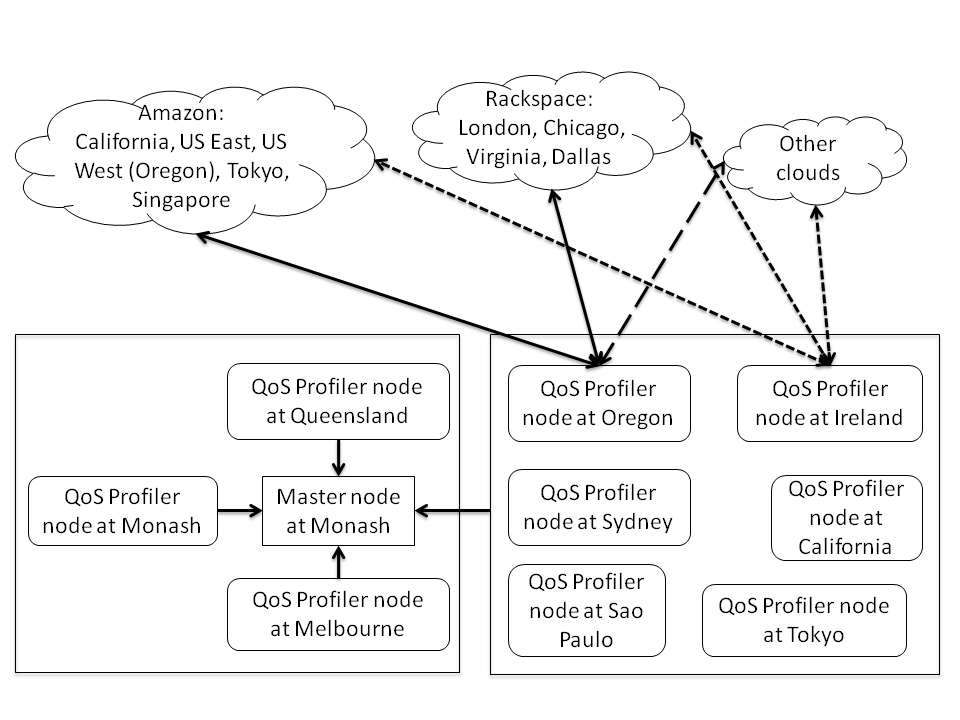
\includegraphics[width=\textwidth,keepaspectratio]{Figures/QoS/figure2.png}
 \caption{QoS Monitoring Service Network Topology. We have used 2 Clouds namely: Nectar Research Cloud and Amazon Web Service. Since Nectar Cloud is free for researchers, we kept the instances running all the time, hence the decision to put master in Nectar. Because there is a limit of quota in Nectar and Amazon have greater geographical coverage in terms of data-center locations. We use additional Spot instance from Amazon as slave data crawlers. A QoS Monitoring Node profiles Download Speed, Latency and Upload Speed at each datacenter in various Clouds from different locations.}
\label{fig:QoSMonitoringServiceNetworkTopology}
\end{figure}

Initially, the QoS data was collected every 2 hours by running the ``speedtest'' service of CloudHarmony. A single run takes more than an hour to finish hence we are collecting it at maximum possible granularity. Later by analyzing the data, we conclude that such high frequency is not necessary, as the average QoS from a particular location to a particular data center most of the time fluctuating between a resealable range. That means the average would be pretty stable. We can use the historical data as a pretty reliable indication. Note that difference between data-centers and various locations are still huge as expected, see Fig. \ref{fig:DownloadSpeedFromAmazonToMelbourne}. In the future we may allow a combination of real time and off-line values to be used if necessary.

\begin{figure}[!ht]
 \centering
 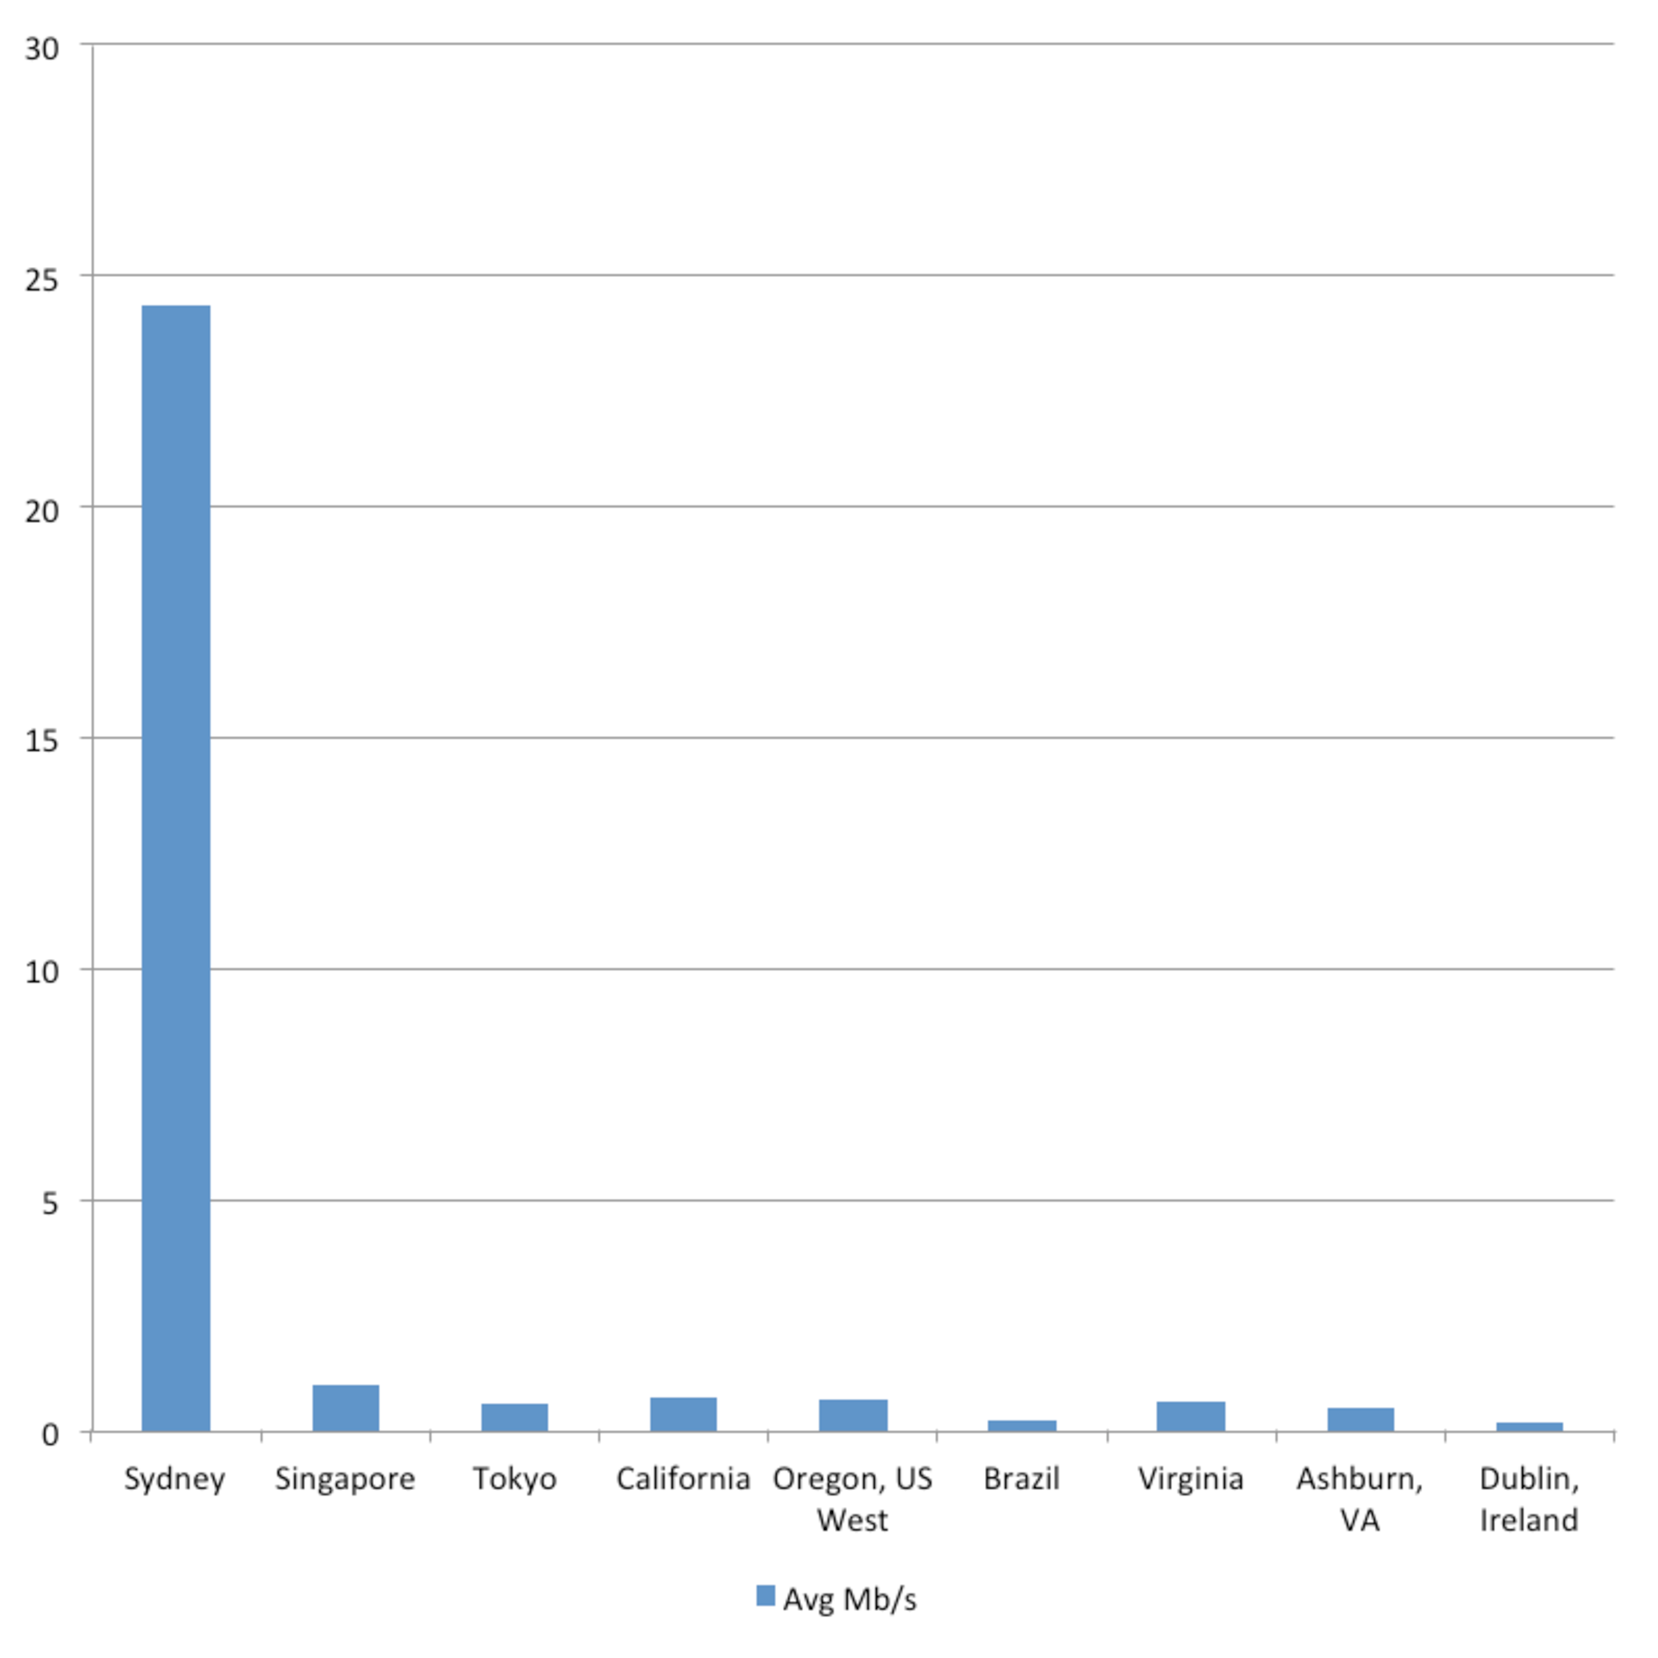
\includegraphics[width=\textwidth,keepaspectratio]{Figures/QoS/figure5.pdf}
 \caption{Download speed from Amazon data centers to Melbourne}
\label{fig:DownloadSpeedFromAmazonToMelbourne}
\end{figure}

Figure \ref{fig:DownloadSpeedFromAmazonToMelbourne} shows that geographically close data center has (as high as 25 times) better network performance, hence this validates the fact that location is one of the important criteria which should be considered during selection process. Our measurements also indicate that distance is not the only factor that effects the network performance, as shown in Fig. \ref{fig:DownloadSpeedAgainstDistance}, data centers are ordered from closest to furthest from left to right, Tokyo and Brazil clearly perform poorly than expected. Hence, we consider the need for active probing and profiling of network QoS from user's endpoint connection to the cloud data centers. By doing so we get clear picture of data centre's network QoS from the users' device that may be deployed across topologically distributed network locations. Note that we have left out Sydney on purpose. Fig \ref{fig:DownloadSpeedFromAmazonToMelbourne} shows the exponential increase in speed between Sydney and Melbourne compare to overseas locations, while Fig \ref{fig:DownloadSpeedAgainstDistance} shows the linear relationship between downloading speed and distance among overseas locations. We are aware that while it is generally true that the geographical distance between any pair of servers (or users) on the Internet affects the route trip time (RTT), the bandwidth between them is not necessarily determined by the distance, many other aspects can affect the user end QoS, like the last-mile home-connecting technology, local Internet traffic condition. Our measurements are only providing suggestive base for further optimisation, user's actual experience will vary.

\begin{figure}[!ht]
 \centering
 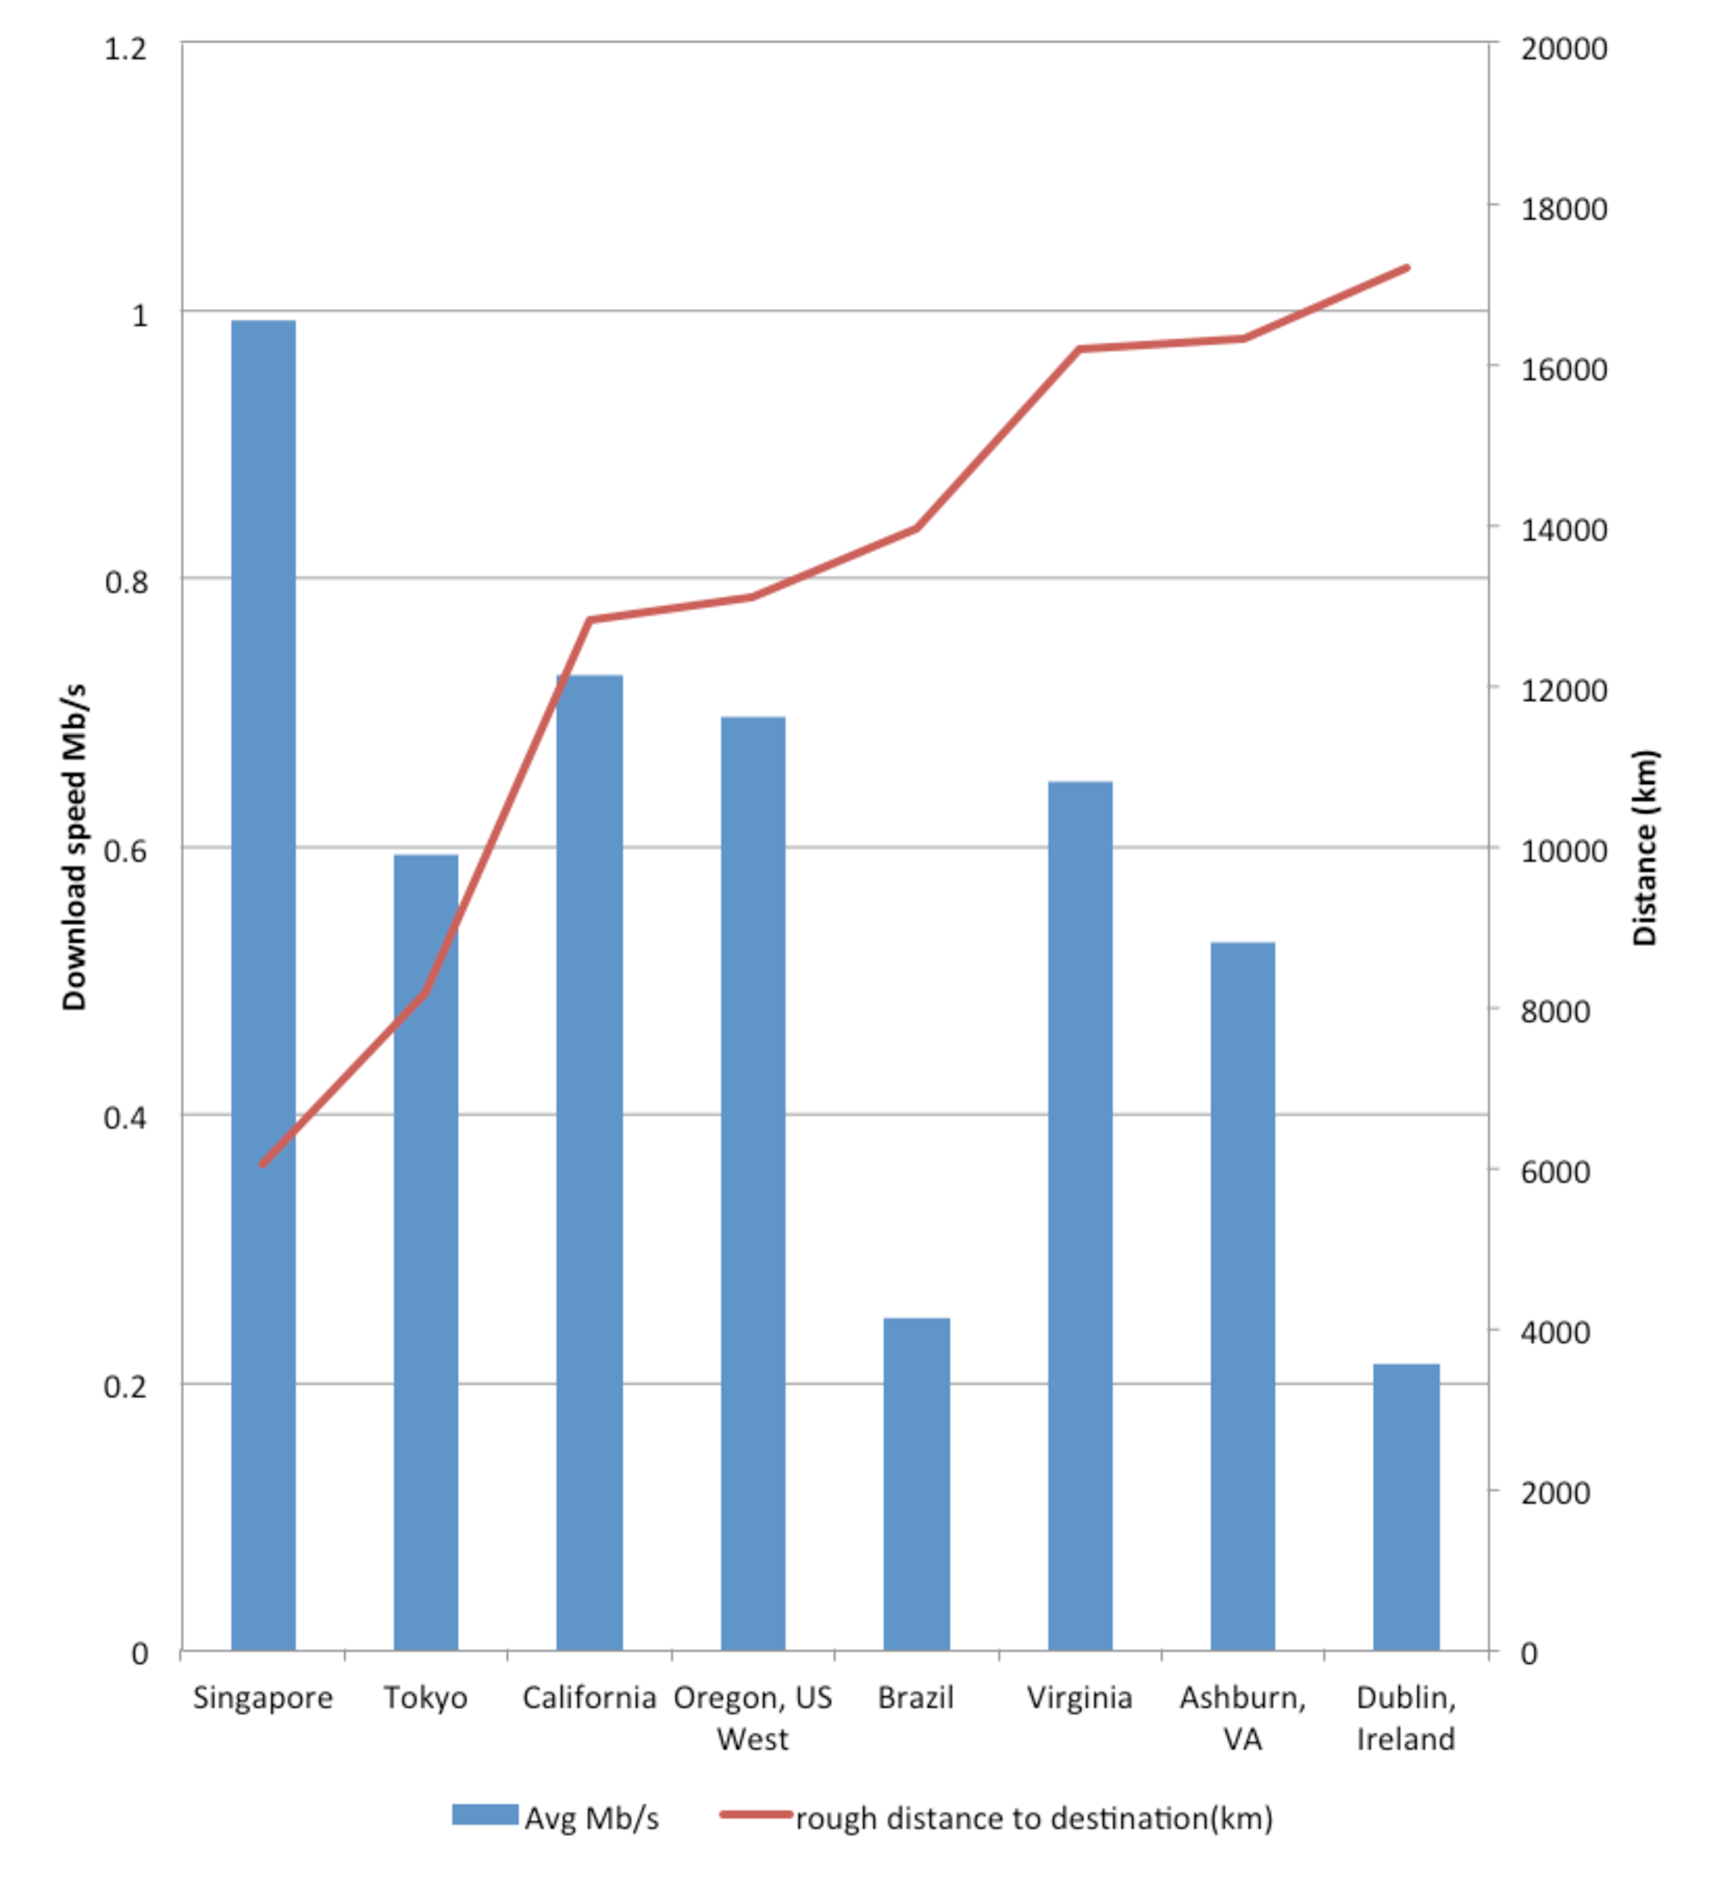
\includegraphics[width=\textwidth,keepaspectratio]{Figures/QoS/figure6.pdf}
 \caption{Download Speed Against Distance.}
\label{fig:DownloadSpeedAgainstDistance}
\end{figure}

\section{Limitation to Existing Approaches}
For research problem described in Section \ref{subsec:service_comparison}, a number of research \cite{Li2010} and commercial projects provide simple cost calculation or benchmarking and status monitoring, but none is capable to consolidate all aspects and provide a comprehensive ranking of infrastructure services.
For instance, CloudHarmony \cite{cloudharmony_speedtest} provides up-to-date benchmark results without considering cost, Cloudorado \cite{Cloudorado} calculates the price of IaaS-level compute services based on static features (e.g., processor type, processor speed, I/O capacity, etc.) while ignoring dynamic QoS features (e.g., latency, throughput, load, utilization).
Yuruware had claimed to have comparison features, but it is no longer available.
Table \ref{table:comparison} shows a brief comparison of the CloudRecommender with other existing products we mentioned previously. We have to clarify that we are more interested in the first 3 features.

To further distinguish ourselves from others, we offer the following two innovative features when ranking, selecting, and comparing various vendor services: 1) allow users to choose to include the QoS requirements during comparison; 2) when users want to take into account mixed qualitative (e.g. hosting region, operating system type) and quantitative criteria, we apply the Analytic Hierarchy Process (AHP) to aggregate numerical measurements and non numerical evaluation. Results are personalized according to each user's preferences, because AHP takes users' perceived relative importance of criteria (pair-wise comparisons) as inputs.

\begin{table}[!ht]
\caption{A Brief Comparison of The Cloud Recommender With Other Existing Solutions}
\label{table:comparison}
\begin{center}
\begin{tabular}{|p{35mm}|p{20mm}|p{25mm}|p{29mm}|p{22mm}|}
\hline
\diagbox{Product}{Feature}&
QoS Benchmark &
Single Criteria Comparison &
Aggregate Ranking Comparison &
Cloud Management\\
\hline
Broker@Cloud & \multicolumn{4}{c|}{No evidence on progress of project}\\
\hline
Yuruware & No & No & No & \cellcolor{light_gray}Yes\\
\hline
CloudHarmony & \cellcolor{light_gray}Adjustable & No & No & No\\
\hline
Cloudorado & No & \cellcolor{light_gray}Yes & No & No\\
\hline
CloudBroker & \cellcolor{light_gray}Adjustable & \cellcolor{light_gray}Yes & No & No\\
\hline
CloudRecommender & \cellcolor{light_gray}Fixed & \cellcolor{light_gray}Yes & \cellcolor{light_gray}Yes & No \\
%\hline \multicolumn{5}{|r|}{Created September 2013}\\
\hline
\end{tabular}
\end{center}
\end{table}

\section{Choosing a Multi Criteria Decision Making Technique}
The selection of cloud service involve weighing the pros and cons of
of multiple criteria,
this is fundamentally a multi criteria decision making problem.
We surveyed some well know MCDM methods in Section \ref{sec:MCDA}.
We chose AHP because it handles multiple criteria,
i.e. capable to optimize mixed qualitative and quantitative criteria.
And AHP doesn't involve complex mathematics, it is very intuitive to use.
In comparison, SAW is strong in single dimensional problems, but not perform as 
good on multi dimensional problems; WPM has a problem dealing with the equal weight of decision matrices. PROMETHEE requires generalized criteria to be defined, such input is difficult for an inexperienced user to provide; the mechanism of VIKOR doesn't fit our problem. 
Furthermore, one problem encountered in most MCDM methods (e.g. TOPSIS) is computation of the weightage of the criteria. This problem is tackled by various ways like AHP, cross-entropy, fuzzy preference programming, etc \cite{AHPvsTOPSIS}.
This also make AHP stand out as a stand along solution, which does not partially depends on other methods.

\section{Ranking with Analytic Hierarchy Process}
We will present how we build a decision making framework based on Analytic Hierarchy Process (AHP) to solve the proposed problems in Section \ref{sec:research_problem}.
It will not only allows users to compare and select a cloud service based on a single criterion (e.g. total cost, max size limit for storage, memory size for compute instance), but also supports a utility function that combines multiple selection criteria pertaining to storage, compute, and network services.
In this chapter we focus on the following topics:

\textbf{1. Problem Formulation.} We first provide a clear formulation of the research problem by identifying the most important cloud service selection criteria relevant to specific real-time QoS-driven applications, selection objectives, and cloud service alternatives.

\textbf{2. Multi-criteria Optimization.} Then illustrations are provided on how AHP based decision (service selection) making technique are implemented. Examples are provided on how to handles multiple quantitative (i.e. numeric) as well as qualitative (descriptive, non numeric, like location, CPU architecture: 32 or 64 bit, operating system) criteria. How pair-wise comparisons can be conducted to determines the relative importance of criteria is also described.

We also developed an decision support tool with the proposed techniques. It will automate and map users' specified application requirements to specific Cloud service configurations. The details and evaluations (conducted in real-world context) are presented in Chapter \ref{cha:system}.

\section{Problem Formulation}
We first provide a clear formulation of the research problem by identifying the most important cloud service selection criteria relevant to specific real-time QoS-driven applications, selection objectives, and cloud service alternatives.

To give a conceptual explanation of our approach to address the QoS optimization problem, we define a formal model in this section. Based on the formal model, we can describe the involved concepts that are incorporated in the algorithm presented later. Particularly, we define a cost estimation function using resource utilization estimations, and a benefit-cost ratio-based evaluation function which considers weights. Furthermore, we present a pair-wise comparison method to calculate normalized weights. For more precise resource utilization estimations, we show how variable resource utilization patterns can be incorporated into cost estimation.

\subsection{Cost Estimation}
Let "a" be the resource usage of a particular resource from a data center location of a Cloud provider. For example, we can use $a_{storage,any,any}=50 GB$ to represent user's need to store 50 GB of data in the cloud. The symbols' meanings are summarized in Table \ref{table:formula_symbols}. Equation \ref{eq:a} means the usage of the compute resource $r$ from provider $c$ at location $l$ is between $0$ and $n$. This value is usually suggested by users. Our assumption is that users may have a rough estimate of how much resources they might need.

\begin{table}[!ht]
\begin{center}\caption{Symbols used in the formulas} \label{table:formula_symbols}
\begin{tabular}{|c|p{10cm}|}
\hline
\textbf{Symbol }&  \textbf{Meaning  }  \\
\hline a & Resource usage behave like a decision variable. \\
\hline C & Set of all possible Cloud providers. \\
\hline c & Cloud Provider, e.g. Amazon,Rackspace, GoGrid. \\
\hline D & Downloading speed. \\
\hline i & Identifies a request. \\
\hline L & Set of all possible datacenter locations. \\
\hline l & A datacenter location, e.g. Sydney, Tokyo. \\
\hline $\zeta$ & Latency (download). \\
\hline  M & Memory Size (e.g. 8G). \\
\hline  P & Price \\
\hline  R & Set of all possible resources, including all types whether it is Compute, Storage or Network.\\
\hline  r & Identifies a source, e.g. GoGrid XX - Large Instance, S3 Storage Serive, EC2 instance.\\
\hline $\gamma $ & $\;$ Set of Requests from one user. \\
\hline  S & Storage. \\
\hline  T & Period of time the resource is used. \\
\hline  t & Exact point in time, like a time stamp. \\
\hline  U & CPU speed. \\
\hline $\mu$ & Uploading speed. \\
\hline w & Weight. \\
\hline
\end{tabular}
\end{center}
\end{table}

\begin{equation}\label{eq:a}
{{\rm{a}}_{r,c,l}} \in \{ 0,1, \ldots ,n\}
\end{equation}
To calculate the Cost (represented by function: $\wp $) for one kind of resource used at one point in time, we multiply its usage with the corresponding unit price (P) as:
\begin{equation}\label{eq:p}
\wp (t) = {a_{r,c,l}}{P_{r,c,l}}
\end{equation}

After initial filtering on which options are appropriate for users, we can calculate the total (minimum) price per unit time for desired resource(s) (assume constant resource usage pattern throughout the time) as in formula \eqref{eq:period_cost}. We assume users will choose the time period (T) they want to estimate price for, e.g. 1 hour, 30 days.
\begin{equation}\label{eq:period_cost}
{a_{r,c,l}}{P_{r,c,l}}{T_{r,c,l}}
\end{equation}

\subsection{Cost Benefit Ratio}
\label{sec:cost_benefit_ratio}
In our decision making framework, we consider the following QoS statistics: download latency ($\zeta$), download speed (D) and upload speed ($\mu$). Those characteristics are important for end-users experience and satisfaction. It's possible to have options that have small price difference, or when having high quality service is more important than saving money. So we offer to calculate the cost/benefit ratio for the resources requested as in \eqref{eq:ratio}.
\begin{equation}\label{eq:ratio}
\frac{ w_1 \sum { a_{c,l,r} P_{c,l,r} T_{c,l,r} } + w_2 \bar\zeta_{c,l,r} } {w_3 \bar\mu_{c,l,r} + w_4\bar D_{c,l,r}}
\end{equation}

Since users are likely to select a combination of compute storage and network services, hence the summation over resources when calculating the cost.

Note that the network QoS of Compute and Storage Service are both collected then separately stored, since user maybe only interested in one of the services. For example, transferring files from (and to) the compute instance relatively ``local"  mounted storage is different from downloading or uploading files from/to dedicated storage only service (like AWS S3 \cite{S3}). In case user select both, we use the average. For instance, in the equation we used $\bar D$ to denote that we take the average of $D_{compute}$(download speed measured from the Compute service) and $D_{storage}$  (download speed measured from the Storage service).

Symbol w represents the weight, which measures users' perceived importance on a parameter, and $w_{1}+ w_{2}=1$ and $w_3+ w_4=1$ means the sum of the weights of benefits and cost each equals to one. Fig. \ref{fig4} shows the criteria to be optimized. They are categorized into two groups: to be maximized or to be minimized.

\begin{figure}[!ht]
 \centering
 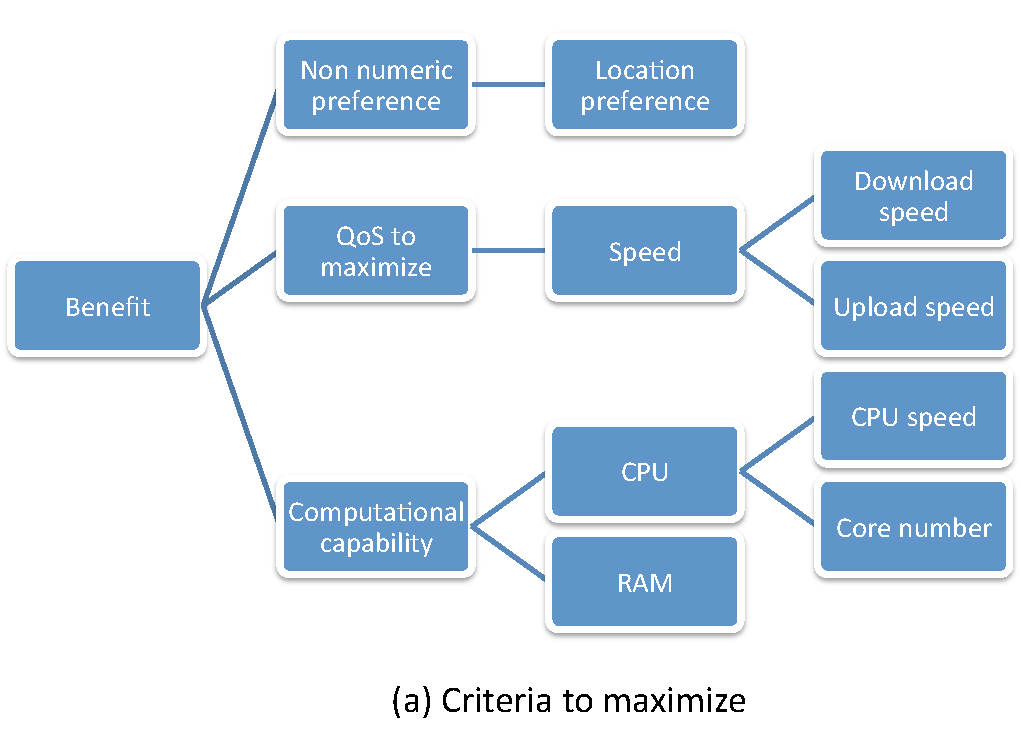
\includegraphics[width=\textwidth,keepaspectratio]{Figures/AHP/figure4a.pdf}
  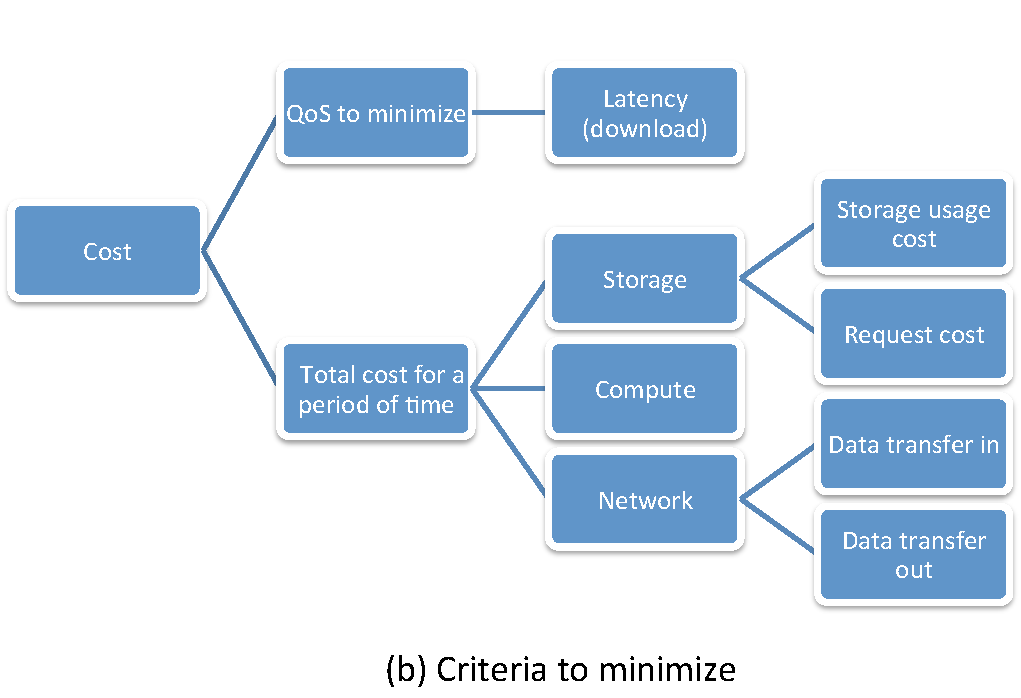
\includegraphics[width=\textwidth,keepaspectratio]{Figures/AHP/figure4b.pdf}
 \caption{ Criteria taken into consideration during comparison. There are 2 categories: benefit and cost. ``Benefit" groups the ``good" criteria which are meant to be maximized. Similarly, ``Cost" groups the ``bad" criteria to be minimized. The actual values to be collected and stored are at the ``leaf" (i.e. Node/criterion with no children) of the ``tree". For example, under ``Benefit", numeric values are collected for ``Download/Upload Speed", ``CPU Speed" and ``Number of Cores". ``QoS to Maximize" is the parent/big category ``Download/Upload Speed" belongs to, there is no value stored for this node.}
\label{fig4}
\end{figure}

As we named this ratio ``Cost Benefit Ratio'', we put cost on the numerator and benefit in the denominator. As a result we will be looking for smaller ratio as better option. Reversing numerator and denominator can still work, just means bigger ratios indicating better option.

\subsection{Weight computed by Pairwise Comparison}
\label{sec:weight&pairwise_comparison}
The weight is calculated based on AHP's pair wise comparison method. We choose the commonly used scale    \cite{ghodsypour1998decision}   \cite{haas2005illustrated} shown in Table \ref{table:scale}. In case user chooses to treat all options equally, equation \eqref{eq:ratio} becomes \eqref{eq:ratio_eq_weight}.

\begin{equation}\label{eq:ratio_eq_weight}
\frac{ 0.5\sum {{a_{r,c,l}}{P_{r,c,l}}{T_{r,c,l}}} + 0.5{\zeta_{c,l,r} }}{{ 0.5{{\bar \mu }_{c,l,r}} + 0.5{{\bar D}_{c,l,r}}}}
\end{equation}

\begin{table}[!ht]
\begin{center}\caption{ABSOLUTE VALUE AND CORRESPONDING DESCRIPTIVE SCALE REPRESENTING RELATIVE IMPORTANCE} \label{table:scale}
\begin{tabular}{|c|c|c|}
\hline
\textbf{Scale }&  \textbf{Value } & Reciprocals\tnote{1}$*$ \\
\hline equal & 1 & 1\\
\hline moderate & 3 & 1/3 \\
\hline strong & 5 & 1/5 \\
\hline very strong & 7 & 1/7 \\
\hline extreme & 9 & 1/9\\
\hline
\end{tabular}
\begin{tablenotes}
  \item[1] $*$If activity i has one of the above nonzero numbers assigned to it when compared with activity j, then j has the reciprocal value when compared with i.
\end{tablenotes}
\end{center}
\end{table}

Otherwise, weight is calculated as shown in Table \ref{table:weight}. 
The meaning of symbols is explained in Table \ref{table:weight_explanation_symbols}.

\begin{table*}[!ht]
\begin{center}
\caption{Matrix Illustrating How To Turn Pair-wise Preference Into Global Weight.}
\label{table:weight}
\begin{tabular}{ccccccc}
& $V_{speed_{upload}}$ & $V_{speed_{download}}$ & $V_{ram}$ & $V_{compute_{disk}}$ & Row Sum & Weight \\
$V_{speed_{upload}}$ & 1 & ${x_{1}}$ & ${x_{2}}$ & ${x_{3}}$ & ${y_{1}}$ & ${y_1}/\tau$  \\
$V_{speed_{download}}$ & $1/{x_1}$ & 1  & ${x_{4}}$ & ${x_{5}}$ & ${y_{2}}$ & ${y_2}/\tau$  \\
$V_{ram}$ & $1/{x_2}$ & $1/{x_4}$ & 1 & ${x_{6}}$ & ${y_{3}}$ & ${y_3}/\tau$ \\
$V_{compute_{disk}}$ & $1/{x_3}$ & $1/{x_5}$ & $1/{x_{6}}$ & 1 & ${y_{4}}$ & ${y_4}/\tau$ \\
& & & & Column Sum & $\tau$ & 1\\
\end{tabular}
\end{center}
\end{table*}

\begin{table}[!ht]
\begin{center}\caption{Symbols Used In Weight Explanation.} \label{table:weight_explanation_symbols}
\begin{tabular}{|c|c|c|}
\hline
\textbf{Symbol }&  \textbf{Meaning } \\
%\textbf{benchmark }& \textbf{mode} &
%\textbf{ mode}  & \textbf{ mode}\\
\hline $\tau $ & $\sum\limits_{n = 1}^{n = 4} {{y_n}} $ \\
\hline V & Value given by User to rate the importance. \\
\hline $V_{compute_{disk}}$ & How important is the size of disk space on VM. \\
\hline $V_{cost}$ & Importance value for cost. \\
\hline ${V_{latency}}$ & Importance value for Download Latency. \\
\hline $V_{ram}$ & How important is the size of memory allocated to VM. \\
\hline $V_{speed_{upload}}$ & Importance value for Upload Speed. \\
\hline $V_{speed_{download}}$ & Importance value for Download Speed. \\
\hline x & Some user input value. \\
\hline y & Sum of the row values. \\
\hline ${y_1}$ & $\left( {\sum\limits_{n = 1}^{n = 3} {{x_n}} } \right) + 1$ \\
\hline ${y_2}$ & $\left( {\sum\limits_{n = 4}^{n = 5} {{x_n}} } \right) + 1 + \frac{1}{{{x_1}}}$\\
\hline
\end{tabular}
\end{center}
\end{table}

\begin{equation}\label{eq:eigenvector}
\left[ \begin{array}{l}
{y_1}/\tau \\
{y_2}/\tau \\
{y_3}/\tau \\
{y_4}/\tau \\
\end{array} \right]
\end{equation}
The fully fledged AHP method consists of repeated matrix squaring to compute the eigenvector, as calculated in \eqref{eq:eigenvector}, every tiny improvement on precision of the eigenvector gained is at the cost of expensive computation, this is supposed to be repeated until no big enough difference (i.e. to four decimal places)  can be observed. In our case, we noticed that the improvement is so small that this rule can be relaxed to omit iterations on matrix squaring.

For example, user may have preference like shown in Table \ref{table:weight_example}. It will produce the preference matrix $M_1$, shown in \eqref{matrix:m1}.
\begin{equation}\label{matrix:m1}
\begin{array}{c}
    M_1\\
    \begin{bmatrix}
        1 & 1/3 & 1/5 & 1/5 \\
        3 & 1   & 3   & 5 \\
        5 & 1/3 & 1   & 3 \\
        5 & 1/5 & 1/3 & 1\\
    \end{bmatrix}
\end{array}
\end{equation}

\begin{table}
\begin{center}
\caption{Example User Preference.}
\label{table:weight_example}
\begin{tabular}{@{}c@{}c@{}c@{}c@{}c@{}}
& $V_{speed_{upload}}$ & $V_{speed_{download}}$ & $V_{ram}$ & $V_{compute_{disk}}$ \\
$V_{speed_{upload}}$ & 1 & 1/3 & 1/5 & 1/5 \\
$V_{speed_{download}}$ & & 1 & 3 & 5 \\
$V_{ram}$ & & & 1 & 3 \\
$V_{compute_{disk}}$ & & & & 1 \\
\end{tabular}
\end{center}
\end{table}

Table \ref{table:example_eigenvector} shows the steps breakdown to compute the eigenvector from \eqref{matrix:m1} before matrix squaring.

\begin{table}[ht]
\begin{center}
\caption{Example Eigenvector Calculation.}
\label{table:example_eigenvector}
\begin{tabular}{cccccccccc}
          &   &        &   &        &   &     &            & Row Sum \\
        1 & + & 0.3333 & + & 0.2    & + & 0.2 & =          & 1.7333  \\
        3 & + & 1      & + & 3      & + & 5   & =          & 13      \\
        5 & + & 0.3333 & + & 1      & + & 3   & =          & 9.3333  \\
        5 & + & 0.2    & + & 0.3333 & + & 1   & =          & 6.5333  \\
          &   &        &   &        &   &     & Column Sum & 30.5999 \\        
\end{tabular}
\end{center}
\end{table}

The result eigenvector would be \eqref{eq:eigenvector1}.
\begin{equation}
\label{eq:eigenvector1}
v_1=
\left[ 
\begin{array}{c} 
0.0566 \\ 
0.4248 \\
0.3050 \\
0.2135
\end{array} 
\right] 
\end{equation}

If we square the matrix \eqref{matrix:m1} we get \eqref{eq:m1square}.
\begin{equation}
\label{eq:m1square}
\begin{array}{c}
    M_1 \times M_1 =
    \begin{bmatrix}
        4      & 58/75 & 22/15  & 8/3 \\
        46     & 4     & 124/15 & 98/5 \\
        26     & 44/15 & 4      & 26/3 \\
        184/15 & 98/45 & 34/15  & 4\\
    \end{bmatrix}\\
\end{array}
\end{equation}

The eigenvector calculated from \eqref{eq:m1square} is \eqref{eq:eigenvector2}.
\begin{equation}
\label{eq:eigenvector2}
\left[ 
\begin{array}{c} 
0.0597 \\ 
0.5223 \\
0.279 \\
0.1389
\end{array} 
\right] 
\end{equation}

The change of value in the new eigenvector is vary small, hence why we decide to omit this step and just use the original weight values ($v_1$). And we assume the preference for cost and latency are 0.8 and 0.2, so we can calculate the overall rank as shown in \eqref{eq:ratio_example}.
\begin{equation}\label{eq:ratio_example}
\frac{0.8 \sum { a_{c,l,r} P_{c,l,r} T_{c,l,r} } + 0.2 \bar\zeta_{c,l,r} }{0.0566 \bar\mu_{c,l,r} + 0.4248\bar D_{c,l,r} + 0.3050 \sum M_{c,l,r} + 0.2135 \sum S_{c,l,r}}
\end{equation}
Where $M$ represents memory size and $S$ is storage size.

\section{Algorithm}
It's more likely that users choose to use a single provider to eliminate costly cross-provider data transfer, but others may have the need to use multiple providers to achieve greater coverage and disaster resilience.

We have abstract our approach in Algorithm \ref{algo:orderedSolutions}. Most of the symbols can be found in Table \ref{table:algo_symbols} and \ref{table:relational_algebra_set}, some symbols are defined earlier in Table \ref{table:formula_symbols} and \ref{table:weight_explanation_symbols}. We have separated the relational algebra and set operations into Table \ref{table:relational_algebra_set}, please pay attention to operation G as it has multiple inputs represented by superscript and subscripts.

\begin{table}[!ht]
\begin{center}\caption{Symbols Used In Algorithm.} \label{table:algo_symbols}
\begin{tabular}{|c|p{10cm}|}
\hline
\textbf{Symbol }&  \textbf{Meaning} \\
\hline AvgQoS &   Table/Relation contains the QoS data collected \\
\hline ${D_{compute}}$ &   Download speed from the compute instance \\
\hline ${D_{storage}}$ &   Download speed from pure storage, i.e. S3 \\
\hline $\bar D$ &   Average download speed calculated as: $\frac{1}{2}\left( {{D_{{\rm{compute}}}} + {D_{storage}}} \right)$ \\
\hline $\ell$ &  
$\ell  \subseteq L$  Some set of locations which are specified by the user, by default 
 $\ell  = L$, which means consider all locations available.
 \\
\hline $M_{min}$ & Minimum memory requirements of compute instance/server  \\
\hline $pric{e_{\max }}$ &   The maximum price one is willing to spend \\
\hline $\rho$ &   
$\rho  \subseteq C$ Some set of  Cloud  providers which are specified by  the user; by
default   $\rho  \subseteq C$, which means consider all locations available. \\
\hline ${\Re _{compute}}$ &  Table/Relation contains all data collected about Compute resources.  \\
\hline ${\Re _{network}}$ &  Table/Relation contains all data collected about Network resource. \\
\hline ${\Re _{storage}}$ & Table/Relation contains all data collected about Storage resource. \\
\hline $\bar \mu $ &   Average upload speed, similar to $\bar D$ \\
\hline U & A tuple representing the estimated usages provided by user, containing the
following: $( U_{compute} , U_{storage} , U_{data_{in}} , U_{data_{out}} )$\\
\hline W & A tuple representing the preference/weight given to each component by the user, it consists of the following: 
$( W_{compute} , W_{storage}, W_{network} $ , $ W_{download} , W_{upload}, W_{latency} )$ \\
\hline
\end{tabular}
\end{center}
\end{table}

\begin{table}[!ht]
\begin{center}\caption{Symbols Used In Algorithm: Relational Algebra and Set Operations.} \label{table:relational_algebra_set}
\begin{tabular}{|c|p{10cm}|}
\hline
\textbf{Symbol }& \textbf{Meaning } \\
\hline 
G & 
    Aggregation operation over a schema, like a \textbf{group by} clause in SQL.
    It follows the format:
    $\tensor[_{a_g}]{G}{_{agg\_op(attri)}} (r)$
    where $a_g$ is the grouping attribute.
    $agg\_op(attri)$ is the aggregation operation over attribute (attri). 
    There are five aggregate functions that are included with most relational database systems.
    These operations are Sum, Count, Average, Maximum and Minimum.
    \textbf{r} is an arbitrary relation.
    See relationa algebra wiki page \cite{ref36} for more details.\\
    
\hline $\sigma $ &  Selection, see wiki page \cite{ref36}.\\
\hline $\bowtie$ & Natural join: depends on the condition can be either $\theta$-join or equijoin. For example, $\bowtie(Provider,Location)$ means equijoin where the condition is join only under the same provider and location\\
\hline  $ \cup$  & Set union operation. \\
\hline $\mapsto $ & Ordered pair, here we use it to denote a new record being formed.\\
\hline
\end{tabular}
\end{center}
\end{table}

\begin{algorithm}[float,caption={orderedSolutions $( \ell , {M_{\min }} , price_{\max} , \rho , U , W )$}, label={algo:orderedSolutions}]
//Filtering on the static characteristics
${\Phi _{compute}}: = {\sigma _{provider \in \rho  \wedge location \in \ell  \wedge memory \ge {M_{\min }}}}\left( {{\Re _{compute}}} \right)$

//Link it with QoS statistics.
${\varphi _{compute}}: = {\Phi _{compute}}{{\rm \bowtie}_{provider,location,serviceName}}AvgQoS$
${\Phi _{storage}}: = {\sigma _{provider \in \rho  \wedge location \in \ell  \wedge quot{a_{low}} < {\upsilon _{storage}}}}\left( {{\Re _{storage}}} \right)$

//Calculating storage price for each tier.
storageCostByQuota: = empty list
foreach$\;{\zeta_s} \in {\Phi _{storage}}\;$do
    if$\;quot{a_{\min }}({\zeta_s}) < {U_{storage}}$
        foreach$\;{\zeta_s} \in {\Phi _{storage}}\;$do
            $storageCostByQuota: = storageCostByQuota \cup \left\{ {{\zeta_s} \mapsto quot{a_{\max }}({\zeta_s})} \right\}* unitPrice({\zeta_s})$
        else
            $\begin{array}{l}
                storageCostByQuota: = storageCostByQuota \cup \left\{ {{\zeta_s} \mapsto \left( {{U_{storage}} - quot{a_{\min }}({\zeta_s})} \right)} \right\}*unitPrice({\zeta_s})
            \end{array}$
        end
    end
end

//Combining storage cost in different tiers to get total.
$\begin{array}{l}
storageCost: = \;\;\;\;\;\;\;\;\;\;\;\;\;\;\;\;\;\;\;\;\;\;\;\;\;\;\;\;\;\;\;\;\;\;\;\;\;\;G\;\;\;\;\;\;\;\;\;\;\;\;\;\;\;\;\;\;\;\;\;\;\;\;\;\;\;\;\;\;\;\;(storageCostByQuota)\\
\;\;\;\;\;\;\;\;\;\;\;\;\;\;\;\;\;\;\;\;\;service\_name\& provider\;\;\;\;\;\;\;sum(storage\_\cos t)
\end{array}$
${\varphi _{storage}}: = storageCost{\bowtie_{provider,location,serviceName}}AvgQoS$
${\Phi _{network}}: = {\sigma _{provider \in \rho  \wedge location \in \ell  \wedge quot{a_{low}} < {\upsilon _{storage}}}}({\Re _{network}})$

//Match appropriate Compute Storage and Network options.
$\varphi : = {\varphi _{compute}}{\bowtie_{provider,location,locatio{n_{client}}}}{\varphi _{storage}}{\bowtie_{provider,location}}{\Phi _{network}}$

$totalCost: = empty\;list$
foreach$\;\zeta \in \varphi \;$do
    $totalCost \cup \left\{ {\zeta \mapsto \sum {{U_r}{P_r}} } \right\}$
end

$ranked: = empty\;list$
foreach$\;\zeta \in totalCost\;$do
    $ranked \cup \left\{ {\zeta \mapsto \frac{{\bar \mu {W_{upload}} + \bar D{W_{download}}}}{{\bar \zeta{W_{latency}} + \sum {{W_r}{P_r}} }}} \right\}$
end

return sortOnRankDescending(ranked)
\end{algorithm}

Algorithm \ref{algo:orderedSolutions} only depicts one common use case, other scenario exists but can be solved with a simplified version of the algorithm or with small modification/addition. We will explains these situation in the following paragraphs.

As shown in Algorithm \ref{algo:orderedSolutions}, a user can provide us the following inputs $( \ell , M_{\min } , price_{\max} , \rho , U , W )$. $\ell$ is the set of locations that a user wants to consider, by default we consider all locations. $M_{\min}$ is the minimal memory requirements for the VMs, 0 denotes no memory requirements. $price_{\max}$ is the maximium budget user willing to spend, 0 indicating they are only interested in free services, -1 is used to represent infinity which means there is no budget constrains. $\rho$ is the set of Cloud service providers that a user wants to consider, by default we consider all providers. $U$ represents the the estimated usages of all the resources: $( U_{compute} , U_{storage} , U_{data_{in}} , U_{data_{out}} )$. $U_{compute}$ is the number of instances, $U_{storage}$ is the number of GB of storage will be used. $U_{data_{out}}$ is the amount of outward data transfer in GB from cloud provider to end devices/users. Similarly, $U_{data_{in}}$ represents the amount of inward data transfer. All the previously mentioned usage estimations are all monthly based, but other length can be used such as daily or hourly, as long as all resource are calculated based on the same standard, there should be no effect on the final comparison and ordering. $W$ represents a user's preference, details are explained in Section \ref{sec:cost_benefit_ratio} and \ref{sec:weight&pairwise_comparison}.

Once options satisfy user requirements have been identified, we calculating price according to different model. There are various pricing models    \cite{weinman2011axiomatic} exist, for example, free, flat-rate, two-part tariffs (like the AWS reserved instance), block-declining (S3 storage), bidding (AWS spot instance). They can mostly be incorporated into our model except the bidding type. One provider often have multiple offers within the same type of services, for example, different kind of instances for the compute service, different storage options, we combine them to get a combinatorial number of choices, we do that for all providers, then calculate the summed cost and rank for each combined option. Not all users need all 3 types of resources, if they specify 0 for a type of resource, it will not be considered. But network service is always needed.

\section{Experiment}
\subsection{Setup}
We run our system and proposed algorithmic technique across a range of hardware systems to understand the implication of hardware resource configuration (see Table \ref{table:experiment_env}) on the performance of the approach.

\begin{table}[!ht]
\begin{center}\caption{Experiment Environments} \label{table:experiment_env}
\begin{tabular}{|p{5mm}|p{30mm}|p{25mm}|p{15mm}|p{25mm}|>{\hspace{0pt}}p{15mm}|}
\hline
\rotatebox[origin=c]{90}{\textbf{Environment}} &  \textbf{Description } &  \textbf{Processor Speed }&  \textbf{Memory}&  \textbf{Processor Name }&  \textbf{Role }\\
%\textbf{benchmark }& \textbf{mode} &
%\textbf{ mode}  & \textbf{ mode}\\
\hline
1 & MacBook Air Physical machine &    1.4 GHz &  2 GB &  $\;$ Intel Core 2 Duo & Master  \\
\hline
2 & Ubuntu 12.04.3 LTS instance ina virtualized environment & 2.4 GHz (1vCPU) & 4 GB & AMD Opteron (TM) Processor 6234 & Master / Profiler\\
\hline
3 & Standard Small (m1.small)Linux / UNIX EC2 Spot Instance & 1.79 GHz ( 1ECU / vCPU) & 1.7 GB & Intel(R) Xeon(R)CPU E5-2650 & Profiler\\
\hline
4 & Compute Optimized(c3.8xlarge) Linux/UNIX EC2Spot Instance & 2.8 GHz (32 vCPU 1081 ECU) & 60 GB & Intel(R) Xeon(R)CPU E5-2680v2 & Performance Testing \\
\hline
\end{tabular}
\end{center}
\end{table}

To summarize, Environment 1 is the local machine used during the development of the program, which is capable of running the database and other system modules.

Environment 2 is the server from The National eResearch Collaboration Tools and Resources (NeCTAR) cloud \cite{NeCTAR} where the our system can be deployed as a service which is easily accessible over the Internet. It is a virtualized environment, so the CPU speed labeled may not accurately reflect the actual allocation.
NeCTAR's infrastructures are located at at eight different organisations (node sites) around Australia. It operates as one cloud system under the Openstack framework. This makes it having different UI and API compare to AWS. Being a collaborative research cloud, it's only open to affiliated members (i.e. Australian researchers, students from participating university). Although the access is free, there is a limitation of 2 instance per member and a cap on the total resource usage. 

Environment 3 is the spot instance type (from Amazon) we used to collect QoS statistics from additional locations, but to cut down the cost; we kept the usage minimal.

Environment 4 is the compute optimized spot instance type we used to test program performance under a powerful CPU, or vertical scalability in short.

\subsection{Case Study}
\subsubsection{Input Parameters}
Table \ref{table:input_param} shows the primary configurable parameters of our algorithm. Everyone's requirements regarding the compulsory parameters usually vary. So we choose a range of values to mimic different selection scenarios. In future work, we may conduct user survey to understand the most concerned factors for different type of users, for example we can exposed all possible constrainable parameters via the API but it may not be necessary (not to mention also slows down the processing) and it will only overwhelm the users who only uses the visual interface. Optional parameters are the one tend to be hard to specify (especially for users with less technical background). Default value column shows what we use when not specified.

\begin{table}[!ht]
\begin{center}\caption{Input Parameters.} \label{table:input_param}
\begin{tabular}{|l|r|}
\hline
\textbf{Compulsory }&  \textbf{Example Value } \\
%\textbf{benchmark }& \textbf{mode} &
%\textbf{ mode}  & \textbf{ mode}\\
\hline Storage(GB/30 Days) & 20 \\
\hline Outbound Data Transfer(GB/30 Days) & 50 \\
\hline Min RAM(GB) & 4 \\
\hline \textbf{Optional } & \textbf{Default Value} \\
\hline Provider Brand & Consider All \\
\hline Display Currency  & AUD \\

\hline Number of Hours to run (per Month) & 720 \\
\hline Number of Instance needed (per Month) & 1 \\
\hline Inbound Data Transfer(GB/30 Days) & 1  \\
\hline Weight of Compute Cost(percentile) & $35\%$ \\
\hline Weight of Storage Cost(percentile) & $25\%$ \\
\hline Weight of Network Cost(percentile) &  $35\%$\\
\hline Weight of Latency(percentile) & $5\%$ \\
\hline Weight of Download Speed(percentile) & $70\%$ \\
\hline Weight of Upload Speed(percentile) & $30\%$ \\
\hline Max RAM(GB) & $100\%$ \\

\hline
\end{tabular}
\end{center}
\end{table}

\subsubsection{Results}
Figure \ref{fig7} shows the top $5\%$ of the result we get from the inputs in Table \ref{table:input_param}. It is in ascending order of ratio (cost over benefit) as indicated by the dotted (blue) line, because lower cost over higher benefit gives us a smaller ratio which representing a better choice.  If we look at ranking by considering only the cost, as illustrated by the solid (red) line, the GoGrid offers dominate over Windows offerings. If to order results in ascending price order (means network QoS constraints are not considered), shown in Fig. \ref{fig8}, Azure disappears from the top $10\%$ of choices. Similarly, we can see that although the price change is small in solutions, their overall rankings are greatly different (dotted blue line). What this means to users is that while we can save money by ignoring network QoS but then they should be ready for degraded network performance Note that although we tried out best in using real world data, sometimes cloud providers vary their prices as frequent as weekly. However, in future work we intend to implement a price crawler service that will automatically parse the provider's web pages and update our system's database.

\begin{figure*}[!htp]
 \centering
 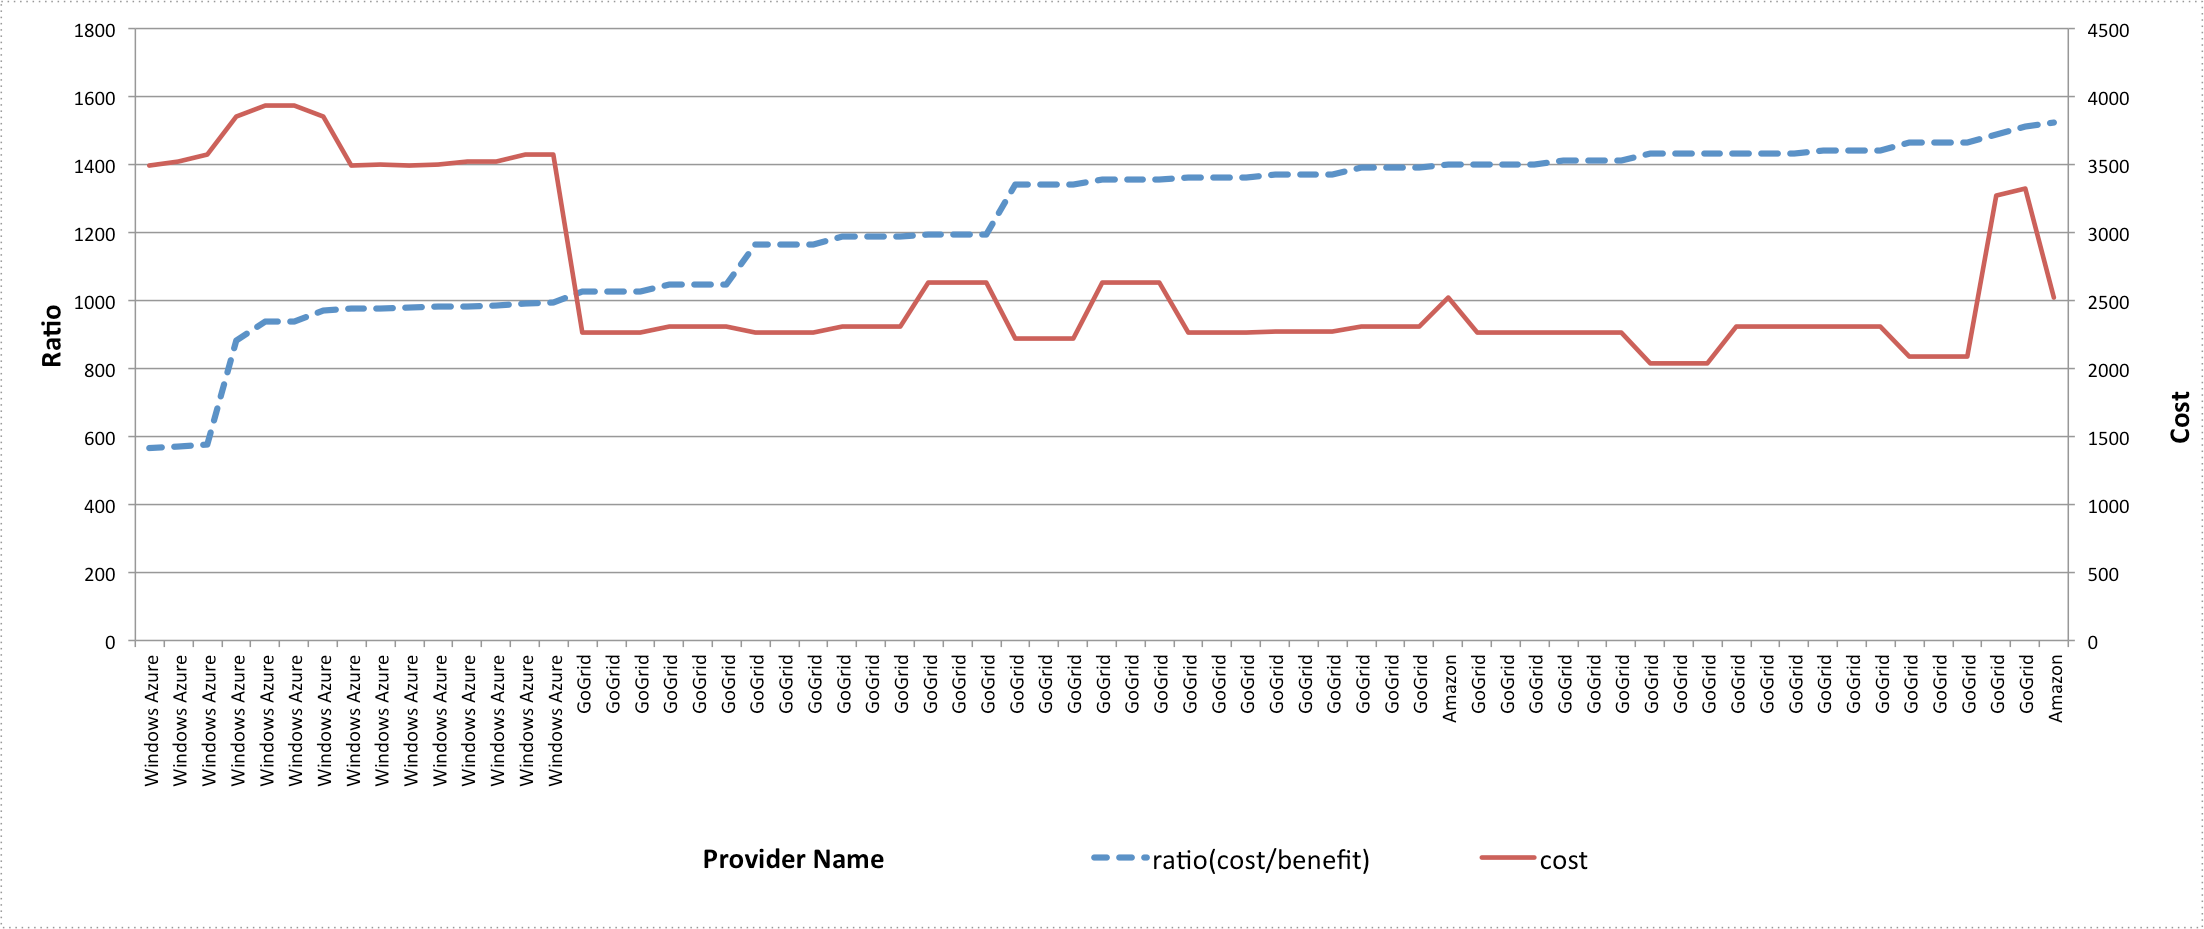
\includegraphics[width=\textwidth,keepaspectratio]{Figures/AHP/figure7.pdf}
 \caption{Results in ascending order by (cost / benefit) ratio}
\label{fig7}
\end{figure*}

\begin{figure*}[!htp]
 \centering
 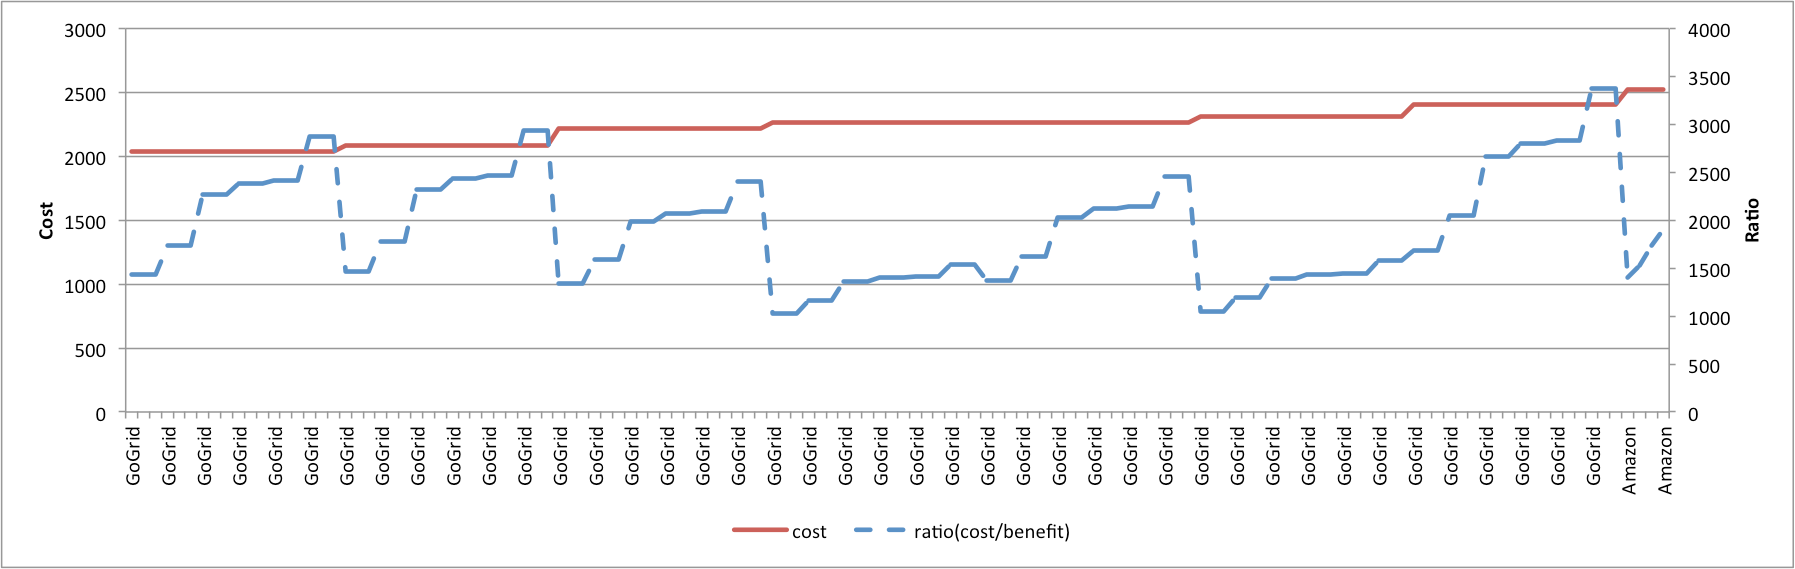
\includegraphics[width=\textwidth,keepaspectratio]{Figures/AHP/figure8.pdf}
 \caption{Results in ascending order by cost}
\label{fig8}
\end{figure*}

\subsubsection{Performance}
The average run time for our current solution is about 11 seconds, with cache turned on in MySQL, we get up to $9\%$ improvement on the same query. As the constraints become stricter the solution space reduces, as a result processing time decreases (to as low as 4.97 seconds), see Table \ref{table:avg_runtime}.

\begin{table}[htbp]
\begin{center}\caption{Average Runtime.} \label{table:avg_runtime}
\begin{tabularx}{\textwidth}{|X|X|p{2cm}|X|X|X|X|X|}
\hline
Test Number &Storage (GB/30 Days) &Outbound Data Transfer (GB/30 Days) & Min RAM (GB) &  Row(s) & \rotatebox[origin=c]{90}{Enviroment 1} &\rotatebox[origin=c]{90}{Enviroment 2} &\rotatebox[origin=c]{90}{Enviroment 4}\\
\hline 1 & 20 & 10 & 0 & 3808 & 12.04 & 11.07 & 10.96   \\
\hline 2 & 40 & 15 & 0 & 3808 & 11.913 & 11.59 & 7.81\\
\hline 3 & 10 & 2 & 0 & 3808 & 11.169 & 10.76 & 7.05 \\
\hline 4 & 20 & 2 & 0  & 3808 & 11.744 & 11.15 & 7.57 \\
\hline 5 & 200 & 200 & 0  & 3808 & 11.894 & 11.72 & 7.49 \\
\hline 6 & 200 & 200 & 0  & 3808 & 11.912 & 10.85 & 6.76 \\
\hline 7 & 200 & 200 & 16  & 552 & 9.15 & 7.7 & 4.97 \\
\hline 8 & 200 & 200 & 8  & 1524 & 9.644& 9.69 & 5.53 \\
\hline 9 & 200 & 200 & 4  & 2095 & 10.25 & 8.72 & 5.58 \\
\hline 10 & 20 & 20 & 0  & 3808 & 12.06 & 11.51 & 7.03 \\
\hline \multicolumn{5}{|r|}{Average} & 11.1776 & 10.476 & 7.075\\
\hline
\end{tabularx}
\end{center}
\end{table}

The performance increase observed when we move from environments 1 to 2 then 4 is resulted from an increase of processing power, hence the idea of "scale up". There is a limit to the amount of processing power one core can have, but our solution is single threaded at the moment, there is still room for improvement by utilizing all cores (like environment 4).  In the future we will explore the option of configuring MySQL/InnoDB to use multithreads (Default is 4 and maximum is 64 since MySQL 5.1.38). Then we will decide whether we need to "scale out".

\subsection{Computational Complexity}
We define the upper bound computational complexity of our optimization approach as shown in \eqref{eq:computational_complexity}.
\begin{equation} \label{eq:computational_complexity}
O\left( {\left| R \right| \times \left| C \right| \times \left| L \right| + \left( \frac{(|\nu|-1)|\nu|}{2}\right)} \right)
\end{equation}

In cost estimation, we have to calculate prices for $|R|$ resources, $|C|$ providers, and $|L|$ geographical locations. In case a more complex utilization function is given, the computational complexity may increase.

In our current model, we consider $|v|$= 6, see weight calculation in Table \ref{table:weight}. Hence to determine the weights in the benefit-cost ratio evaluation function, 15 pair-wise comparisons have to be made, unless user choose to use the default values. In both cases this part of the complexity factor is a constant which can be omitted.